\chapter{Simulating dynamics of quantum systems using quantum annealing}
\chaptermark{Simulating dynamics}
\label{chapter:simulating}

One of the leading motivations behind the development of quantum computing
devices is simulating quantum systems intractable by classical computers. But
how far are we from this goal? To answer this question, one might design an
algorithm for conducting such a simulation of a physical system and then test
how it performs on the current generation of quantum computers. In this
chapter, we follow this idea and present a possible approach for simulating
quantum systems (or any time-dependent dynamical system) that can be used with
annealing devices such as D-Wave quantum annealers and similar devices. To
illustrate the working of our algorithm, we simulate the simplest single-qubit
system and demonstrate that already near-term annealing devices are capable of
capturing its dynamics in a narrow regime of parameters. Furthermore, the class
of physics-inspired problem instances proposed in this chapter
can be valuable in benchmarking other (not necessarily quantum) solvers.

\section{Parallel in time simulation of dynamical systems}
Optimization problems that can be solved using quantum annealers exhibit no
time--dependence. Therefore, simulating any time-dependent phenomena using
those devices requires reformulating the problem as one that is static in
nature. In our case, it is possible by enlarging the Hilbert space of the
system under consideration, so that the states of this larger space encode also
temporal information \cite{feynmanclock}.

Let us start by precisely defining the problem we want to address.
Consider an $L$--dimensional real or complex system, whose state at time $t$ is
described by the vector $\ket{\psi(t)}$ evolving according to a differential
equation of the form:
\begin{equation}
  \label{eq:dynamical-system}
  \frac{\partial \ket{\psi(t)}}{\partial t} = K(t) \ket{\psi(t)}.
\end{equation}

Here, $K$ is the so-called Kamiltonian \cite{goldstein2002classical} and can be
any linear operator acting on $\mathbb{R}^L$ or resp. $\mathbb{C}^L$. Observe
that any isolated quantum system can be described by equation
\eqref{eq:dynamical-system}, as putting $K=-\frac{i}{\hbar}H$, where $H$ is its
Hamiltonian, transforms the equation \eqref{eq:dynamical-system} into
Schr\"{o}dinger equation.

Given an initial state, $\ket{\psi(t_0)}$ the equation
\eqref{eq:dynamical-system} admits a unique solution:
\begin{equation}
  \ket{\psi(t)} \coloneqq U(t, t_0) \ket{\psi(t_0)},
\end{equation}
where operator $U(t, t_0)$ is a propagator transforming the initial state of
the system into its state at time $t$ and is given by:
\begin{equation}
  \label{eq:propagator}
  U(t, t_0) = \mathcal{T} \exp \left( \int_{t_0}^t K(\tau)d\tau \right).
\end{equation}
Here, $\mathcal{T}$ denotes the time-ordering operation \cite{chronological}.
Note that in the case when $K(t)$ commutes with $K(t')$ for every $t' \ne t$,
the time-ordering can be omitted. In particular, this is the case if $K$ is
time-independent.

Given the initial state, we are interested in finding the state of the system
at some time $t > t_0$. Numerical methods for solving this problem usually
start by partitioning the interval $[t_0, t]$ into $N$ distinct time points
$t_0 < t_1 < \ldots < t_{N-1} = t$. Then, the desired state $\ket{\psi(t)}$ can
be computed as:
%
\begin{equation}
  \ket{\psi(t)} = U_{N-1} \cdots U_1 \ket{\psi(t_0)},
\end{equation}
%
where $U_i$ is a shorthand notation for $U(t_i, t_{i-1})$. This is purely a
rearrangement of computations, which by itself gives no benefit over applying
$U(t, t_0)$ directly. However, shortening the interval allows for a more
efficient approximation of propagators, which can be done using a variety of
methods, including Suzuki-Trotter approximation \cite{suzuki}, commutator-free
expansion \cite{commutatorfree} or tensor-networks based approaches
\cite{dmrg}.

This procedure, common to many sequential methods, gives a starting point for a
class of the so-called parallel in--time methods based on the Feynman clock
operator. In these approaches, one starts by suitably enlarging the state space
so that it can encode the temporal data \cite{feynmanclock}. This can be done
by considering a tensor product of a state space with the new Hilbert space
spanned by the orthonormal basis $\{\ket{0}, \ket{1}, \ldots, \ket{N-1}\}$.
Then, the following superposition encodes states of the system in all $N$
moments of time:
%
\begin{equation}
  \ket{\Psi} = \sum_{n=0}^{N-1} \ket{n} \otimes \ket{\psi(t_n)}.
\end{equation}
Consider now the following \emph{clock operator} $\clockop$:
\begin{equation}
  \label{eq:clock2}
  \begin{split}
    \clockop
    =
    \sum_{n=0}^{N-2}
    &\ketbra{n+1}{n+1} \otimes I - \ketbra{n+1}{n} \otimes U_n + \\
    &\ketbra{n}{n} \otimes I - \ketbra{n}{n+1}\otimes U_{n}^{\dagger}.
  \end{split}
\end{equation}
One can see that $\ket{\Psi}$ is a solution (although not unique) to the
eigenequation:
\begin{equation}
  \label{eq:clock-eigenequation}
  \clockop \ket{\mathbf{x}} = 0.
\end{equation}
The non--uniqueness of the solution of \eqref{eq:clock-eigenequation} follows
from the fact that the definition of the clock operator $\clockop$ does not
depend on the initial state. We can fix this problem by adding a \emph{penalty}
term $\clockop_0 = \ketbra{0}{0}\otimes(I-\ketbra{\psi_0}{\psi_0})$ to the
left-hand side. The equation to solve becomes then:
\begin{equation}
  \label{eq:clock-eigenequation2}
  (\clockop + \clockop_0) \ket{\mathbf{x}} = 0.
\end{equation}
If one puts $\coefmatrix=\clockop + \ketbra{0}{0} \otimes I$ and $\ket{\Phi} =
  \ket{0}\otimes \ket{\psi_0}$, the equation \eqref{eq:clock-eigenequation2}
becomes:
\begin{equation}
  \label{eq:gsys}
  \coefmatrix \mathbf{x} = \ket{\Phi}.
\end{equation}
Thus, using an approximation of evolution operators, we constructed a system of
linear equations encoding the solution to the equation
\eqref{eq:dynamical-system} under the given initial condition. At this point,
however, it is not possible to solve it using a quantum annealer yet. To do so,
one first needs to convert this system into an optimization problem with
dichotomous variables, which will be the topic of the next section.
\section{Solving systems of linear equations as an optimization problem}
There is a straightforward way of converting equation \eqref{eq:gsys} into an
optimization problem. One can observe that the solution minimizes the norm
$\left\Vert \coefmatrix\ket{\mathbf{x}} - \ket{\Phi}\right\Vert$. Since the
norm is non-negative, it follows that solving equation \eqref{eq:gsys} is
equivalent to the following optimization problem:
\begin{equation}
  \label{eq:optimize_1}
  \ket{\Psi} = \argmin_{\mathbf{x}} f(\mathbf{x}), \quad f({\mathbf x}) = \left\Vert \coefmatrix\ket{\mathbf{x}} - \ket{\Phi}\right\Vert^2.
\end{equation}
However, $f$ in the equation \eqref{eq:optimize_1} is not the only choice of a
target function. If $\coefmatrix$ is positive-definite, one can consider the
following function $h$ instead:
\begin{equation}
  \label{eq:optimize_2}
  h(\mathbf{x})=\frac{1}{2}\bra{\mathbf{x}}\coefmatrix\ket{\mathbf{x}} -
  \braket{\mathbf{x}}{\Phi}.
\end{equation}
Indeed, one can verify that solution to \eqref{eq:gsys} also minimizes $h$ by
computing its gradient and Hessian:
\begin{equation}
  \nabla h(\mathbf{x}) = \coefmatrix\ket{\mathbf{x}}-\ket{\Phi}, \quad \nabla^2 h({\mathbf
    x})=\coefmatrix>0
\end{equation}
Since Hessian is positive and $\ket{\Psi}$ is the only vector at which $\nabla
  h$ vanishes, it follows that $\ket{\Psi}$ is indeed a global minimum of $h$.

\section{Discretizing variables}
Thus far, we have been working with continuous variables. The next necessary
step before solving optimization problems \eqref{eq:optimize_1} and
\eqref{eq:optimize_2} using annealer is converting them in such a way that all
unknowns are dichotomous. To this end, we will follow a strategy presented in
\cite{fixedpoint,chang}. The idea is to express each of the unknown
coefficients of $\ket{\mathbf{x}} = $[$x_1, \ldots, x_{LN}]^T$ in fixed-point
approximation. While this strategy was originally described for real matrices,
it works for complex matrices as well, since one can employ the natural embedding of $\CC$
into $\RR^{2 \times 2}$, $a+bi \mapsto a\hat{I} + ib\ssigma_{y}$. Henceforth, we assume
that the considered systems are real.

If one assumes (binary) order of magnitude of coefficients of
$\mathbf x$ to be $D$ (i.e. $x_i \in [-2^D, 2^D]$ for each $i$), then it can be
approximated up to $R$ bits of precision using the formula:
\begin{equation}
  \label{eq:fixed}
  x_i \approx 2^D \left(2 \sum_{\alpha=0}^{R-1}2^{-\alpha}q_i^{\alpha} -1\right).
\end{equation}
Here variables $q_i^\alpha$ are consecutive bits of the fixed-points expansion
of $x_i$. Note that approximation of $x_i$ in \eqref{eq:fixed} is a linear
combination of its bits, therefore plugging it into optimization problems
\eqref{eq:optimize_1} and \eqref{eq:optimize_2} yields quadratic unconstrained
optimization problems of the form:
\begin{align}
  \label{eq:qubo_f}
  \argmin_{\mathbf{q}} f(\mathbf{q}) = \argmin_{\mathbf{q}} \sum_{i,\alpha} c_i^{\alpha} q_i^r + \sum_{i,j,\alpha,\beta} d_{ij}^{\alpha\beta} q_i^{\alpha} q_j^{\beta} + f_0, \\
  \label{eq:qubo_h}
  \argmin_{\mathbf{q}} h(\mathbf{q}) = \argmin_{\mathbf{q}} \sum_{i,\alpha} a_i^{\alpha} q_i^r + \sum_{i,j,\alpha,\beta} b_{ij}^{\alpha\beta} q_i^{\alpha} q_j^{\beta} + h_0.
\end{align}
Coefficients in equations \eqref{eq:qubo_f} and \eqref{eq:qubo_h} can be
straightforwardly computed by appropriate substitutions into equations
\eqref{eq:optimize_1} and \eqref{eq:optimize_2}. For brevity, here we present
only the formulas for the equation \eqref{eq:qubo_h}, which reads:
\begin{eqnarray}
  \begin{split}
    b_{ij}^{\alpha\beta} &= \coefmatrix_{ij} 2^{1-\alpha-\beta+2D} \\
    a_i^\alpha &= \left( 2^{-\alpha+D}\coefmatrix_{ii} - 2^D\sum_{j}\coefmatrix_{ij}- \Phi_i\right)2^{1-\alpha+D},
    \\
    h_0 &= 2^D\left( 2^{D-1}\sum_{ij}\coefmatrix_{ij}+\sum_i \Phi_i\right).
  \end{split}
  \label{eq:coeff}
\end{eqnarray}

Our approach requires the order of magnitude $D$ and precision $R$ in equation
\eqref{eq:fixed} to be chosen beforehand. Choosing the right $D$ requires
knowledge of the range in which coefficients lie. If its value is too small,
the approximations will fail to capture the most significant bits of the real
solution. On the other hand, choosing $D$ that is too large will result in
wasting variables for encoding insignificant zeros. Fortunately, for many
systems, a suitable $D$ can be determined. For instance, for qubit and
multi-qubit systems, each $x_i$ is bounded by $\pm 1$ which makes $D=0$ the
optimal choice for this case.

QUBOs in the equations \eqref{eq:qubo_f} and \eqref{eq:qubo_h} are defined on
the graph of size $N \cdot R \cdot L$. The number of edges (i.e. non-zero
quadratic terms) depends on the number of non-zero off-diagonal elements of the
matrix $\coefmatrix$. It is interesting to note that the overall density of the
graph is an increasing function of $R$ (bigger precision requires a denser
graph) while, on the other hand, it tends to decrease with increasing $L$.

We converted the original problem of finding the dynamics of the system into a
binary optimization problem suitable for input to the quantum annealer. In the
next section, we will discuss experiments that we performed using D-Wave
2000Q$_{2.1}$ and D-Wave 2000Q$_5$ machines to test the approach we described.
The results we discuss here were originally reported in \cite{parallelintime}.

\section{Parallel-in-time simulations with quantum annealer}
\sectionmark{Parallel-in-time simulations}
\label{sec:parallel-in-time}
Before discussing the results of our experiments, let us focus first on its
design. To exemplify our approach, we chose to simulate the dynamics of a
two-level system with an initial state $\ket{0}$ and a Hamiltonian $\mathcal{H}$:
\begin{equation}
  \mathcal{H} = \frac{\pi}{2}\ssigma_y,
\end{equation}
where $\ssigma_y$ is a Pauli spin operator in the $y$-direction. This particular
choice of Hamiltonian and initial state makes the system suitable for
implementation on present-day quantum annealers for several reasons. One can
easily see that the evolution of the system is real (as opposed to complex),
which halves the number of needed variables. Secondly, for integral time points
$t_0=0, t_1=1, \ldots$ coefficients of the wave function can be expressed
\emph{exactly} using only two bits of precision per coefficient, which further
reduces the number of variables.

\begin{figure}[!h]
  \centering
  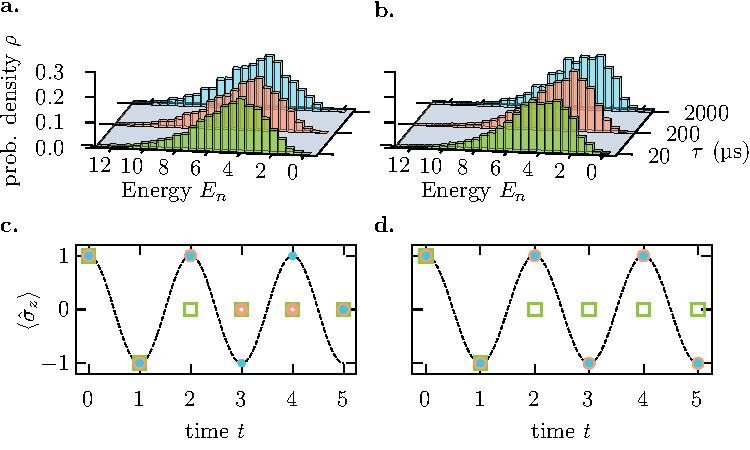
\includegraphics{figures/parallel-dynamics-result.pdf}
  \caption{Results of simulating dynamics of two-level system on D-Wave 2000Q$_{2.1}$
    (left) and low-noise D-Wave 2000Q$_{5}$ (right). \textbf{a.}--\textbf{b.}
    Energy distribution of samples obtained from D-Wave annealers for different
    annealing times $\tau$. Notice a slight shift of distributions towards the
    ground state for the 2000Q$_{5}$ device. \textbf{c.}--\textbf{d.} Rabi
    oscillations of the simulated system. The obtained samples were normed before
    plotting. As can be seen in panel \textbf{d.}, the low-noise device was able to
    faithfully capture oscillations for $\tau=200, 2000$. The annealing time is
    color-coded: $\tau=$ \tikzquad\,\,\, -- 20\textmu{}s, \,\tikzcircle\,\,\,--
    200\textmu{}s, \,\tikzdot\,\,-- 2000\textmu{}s. } \label{fig:energy-hist}
\end{figure}

We simulated the above system using values of $R=2, 3$ and for several numbers
of time points $N$. We used annealing time $\tau$ spanning several orders of
magnitude, namely $\tau=20\mu s$, $200 \mu s$ and $2000 \mu s$. Since the
resulting graphs were dense, we decided to use standard embedding of the
complete graph $K_n$ on Chimera \cite{chimeraclique}. To assess the quality of
solutions obtained from the annealer, we sampled each problem $10^4$ times on
DW-2000Q$_{2.1}$ device as well as its low-noise version, DW-2000Q$_{5}$.
Energy distributions of samples obtained for $N=6$ are depicted in Fig.
\ref{fig:energy-hist}. The same figure also illustrates the dynamics of the
expected value of $\ssigma_z$ for the lowest energy sample obtained for a given
annealing time. Note that to preserve the physical meaning of the decoded
solution, the state vector was normed before plotting.

To put these results into context, we also compare them to the ones obtained
using two purely classical methods: CPLEX optimizer and recently developed
tensor network-based algorithm (which we describe later in Chapter
\ref{chapter:tn}. The results of this comparison are depicted in Fig.
\ref{fig:cplex_tn_dwave}.

\begin{figure}
  \centering
  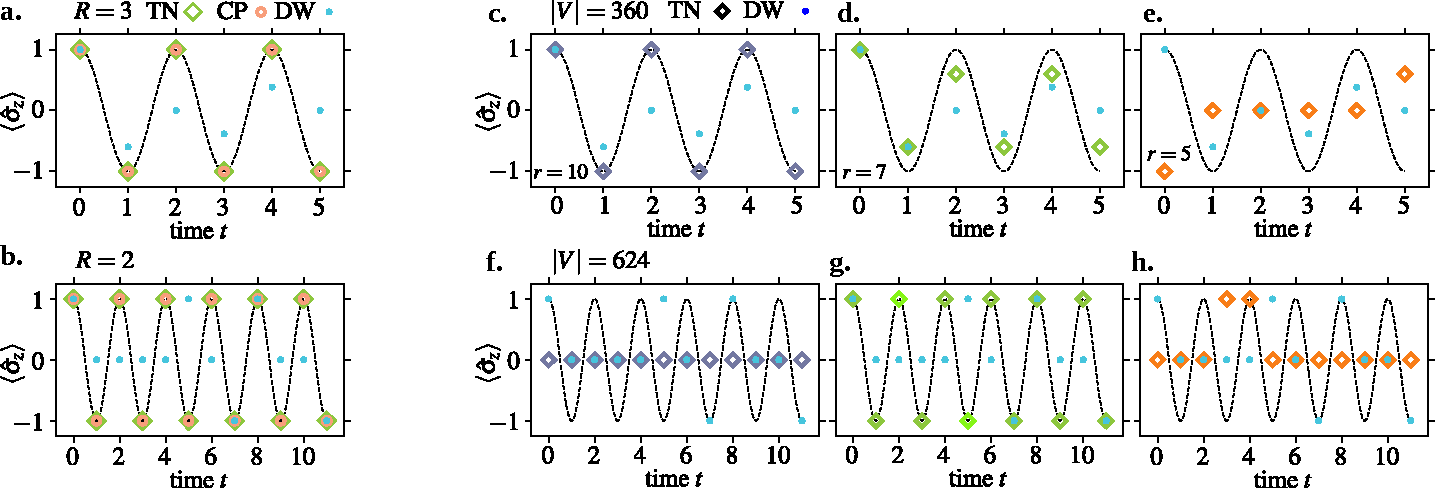
\includegraphics[width=\textwidth]{figures/fig34_merge.pdf}
  \caption{ \textbf{a.}--\textbf{b.} Performance of the two state-of-the-art heuristic
    algorithms: the CPLEX optimizer (CP) and a tensor networks-based (TN) solver
    (see Chapter \ref{chapter:tn}) in comparison to the D-Wave $2000$Q quantum annealer (DW),
    cf. Fig~\ref{fig:energy-hist}. The graphs on which the problems were defined
    had respectively $|V|=360$ (\textbf{a.}) and $|V|=624$ (\textbf{b.}) vertices. The annealing time was set
    to $\tau=200$\textmu{}s. The numerical precision of the solution vector is
    denoted as $R$. %\\
    \textbf{c.}--\textbf{h.} Degradation of the solution quality resulting from perturbing the
    problem by truncating its coefficients to a given
    numerical precision denoted as $r$. The reference ground state obtained
    with tensor networks (TN) is compared to the  experimental data from the
    D-Wave $2000$Q quantum annealer (DW). This effect, expected to be predominant
    in the current quantum annealing technology, is already visible on
    Fig.~\ref{fig:energy-hist}\textbf{a.}--\textbf{d.} and Fig.~\ref{fig:cplex_tn_dwave}\textbf{a.}--\textbf{b.}.
  }
  \label{fig:cplex_tn_dwave}
\end{figure}

Results depicted in figures \ref{fig:energy-hist} and \ref{fig:cplex_tn_dwave}
show that the DW-2000Q$_{5}$ was able to faithfully capture dynamics of qubit
if the state of the system was encoded using $R=2$ bits of precision per
coefficient when the annealing time $\tau=200$ was used. For larger values of
$N$ and $R$ one can observe that the quality of solution degrades. Both CPLEX
and tensor networks-based solvers outperformed D-Wave annealers in terms of the
quality of solutions. The differences were especially noticeable for problem
instances with larger graph sizes, i.e. ones with higher precision ($R \ge 3,
  N=6)$), or with extra time points ($N > 6, R = 2$). The observed degradation of
the solution quality is consistent with the results obtained in other works,
especially for the problems requiring complete graphs, see e.g.
\cite{Hamerly2019}.

\subsection{Discussion of error sources}

The poor performance of D-Wave annealer is something certainly to be expected
from such early-stage devices. Annealers are prone to errors stemming from
multiple sources \cite{dwavedocs}, and it is hard to judge which of those
sources contributed most to the lackluster performance of a particular problem
instance. One of the possible sources of errors is DAC quantization, which
essentially limits the precision of both the quadratic and linear coefficients
passed to the annealer. As a result, the problem that the annealer physically
solves is slightly different than the problem the programmer intended to solve.

One can see that such quantization errors would mostly affect problems with
coefficients lying in close proximity to one another. Indeed, suppose that DAC
quantization errors limit the precision of the linear coefficients to $d$
decimal digits. Then any two coefficients, say $h_{i}, h_{{j}}$ lying closer to
each other than $d$ digits, i.e. $|h_{i} - h_{j}| < 10^{-d}$, become physically
undistinguishable to the annealer. The issue also affects coefficients that are
further apart, by possibly diminishing their relative differences.

While it is hard to pinpoint which source contributed the most to the errors in
the case of the optimization problems discussed in this chapter, we argue that
in our case the poor performance of the annealer can be largely explained by
DAC quantization. Indeed, looking at the \eqref{eq:coeff} one can immediately
see that the optimization problem can contain coefficients arbitrarily close to
each other as long as a large enough $R$ is chosen. To justify this reasoning,
we studied how the tensor network solver performs when the coefficients of the
problem are perturbed by truncating their coefficients to a predefined
number of digits $r$. The results of this experiment are presented in Fig.
\ref{fig:cplex_tn_dwave}\textbf{c.--h.}. One can immediately observe that the
error patterns resemble the ones obtained from D-Wave, which might suggest that
DAC quantization might indeed be a significant source of errors in our case.
However, we would like to point out, that our analysis is by no means
conclusive, and further analysis of error patterns is still needed.

%%% Local Variables:
%%% mode: latex
%%% TeX-master: "../main"
%%% End:
